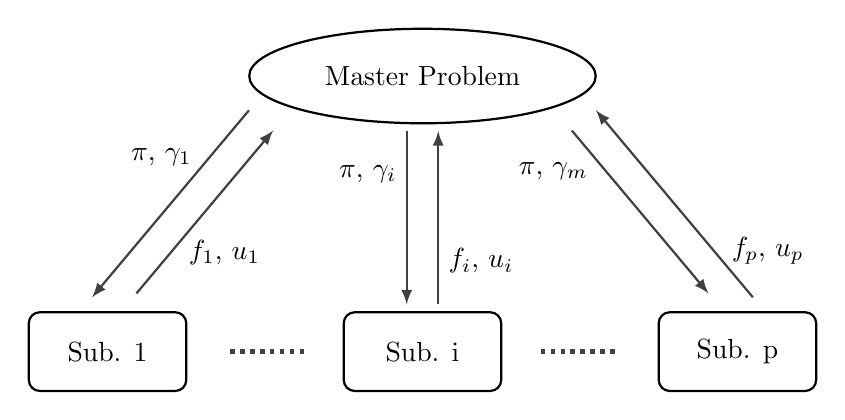
\begin{tikzpicture}

% Ellipse
\draw[thick] (0,0) ellipse(2.2cm and 0.6cm) node[midway]{Master Problem};

% Rectangle i
\begin{scope}[yshift=-4cm]
\draw[thick, rounded corners] (-1,0) rectangle (1,1) node[midway]{Sub. i};
\end{scope}

% Rectangle 1
\begin{scope}[yshift=-4cm, xshift=-4cm]
\draw[thick, rounded corners] (-1,0) rectangle (1,1) node[midway]{Sub. 1};
\end{scope}

% Rectangle p
\begin{scope}[yshift=-4cm, xshift=4cm]
\draw[thick, rounded corners] (-1,0) rectangle (1,1) node[midway]{Sub. p};
\end{scope}

% ith arrows
\draw[-latex,thick,black!75] (-0.2, -0.7) -- (-0.2,-2.9) node[near start,left,black]{\bm{$\pi$}, $\gamma_i$};
\draw[latex-,thick,black!75] (0.2, -0.7) -- (0.2,-2.9)node[near end,right,black]{$f_i$, \bm{$u$}$_i$};

% 1st arrows
\begin{scope}[xshift=-2.5cm]
\begin{scope}[rotate around={-40:(0,-1.1)}]
\draw[-latex,thick,black!75] (-0.2, -0.4) -- (-0.2,-3.5) node[near start,left=0.1cm,black]{\bm{$\pi$}, $\gamma_1$};
\draw[latex-,thick,black!75] (0.2, -0.4) -- (0.2,-3.1)node[near end,right=0.1cm,black]{$f_1$, \bm{$u$}$_1$};
\end{scope}
\end{scope}

% pth arrows
\begin{scope}[xshift=2.5cm]
\begin{scope}[rotate around={40:(0,-1.1)}]
\draw[-latex,thick,black!75] (-0.2, -0.4) -- (-0.2,-3.1) node[near start,left=0.1cm,black]{\bm{$\pi$}, $\gamma_m$};
\draw[latex-,thick,black!75] (0.2, -0.4) -- (0.2,-3.5)node[near end,right=0.1cm,black]{$f_p$, \bm{$u$}$_p$};
\end{scope}
\end{scope}

% Dotted line
\draw[dotted, ultra thick, black!75] (1.5,-3.5) -- (2.5,-3.5);
\draw[dotted, ultra thick, black!75] (-1.5,-3.5) -- (-2.5,-3.5);

\end{tikzpicture}